\chapter{Implementation}

\section{Authentication Policy}
With regard to the design of the authentication policies, conditional flows are used to fulfill the requirements for authentication policies.
The main difference is the additional lifecycle management provided for them with particular validations.
Reusing existing components is beneficial in this case as the implementation is simplified without introducing any other similar components.

In order to differentiate authentication flow and authentication policy, the parent authentication flow \textit{Authentication policies - PARENT} is provided to contain only authentication policies.
Moreover, every policy has the prefix \textit{"POLICY - "} for its alias to mark it as the authentication policy.
The validation and management for authentication policies are done through the specific \textit{Data Access Object} (DAO), shown in Section \ref{impl-authn-policies-dao}. 

As the authentication policies need to be managed from the outside world, the \textit{REST API} has been introduced with a detailed description in Section \ref{impl-authn-policies-rest}.
The administrator console, as a client application, also uses the Keycloak REST API to manage all entities.
More details about the administrator console interface are in Section \ref{impl-authn-policies-admin}.

\begin{figure}[htbp]
  \centering
  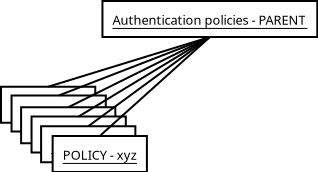
\includegraphics[width=0.5\textwidth]{img/sections/6-implementation/auth-policies-parent.png}
  \caption{Authentication Policies Parent}
  \label{fig:impl-authn-policies-parent}
\end{figure}

\newpage

\subsection{Data Access Object} \label{impl-authn-policies-dao}
A Data Access Object (DAO) pattern in software engineering abstracts database operations, shielding application logic from database sophistication and adhering to the single responsibility principle.\cite{impl-dao}

It is used to manage authentication policies as part of the separation from the authentication flows.
It provides necessary validation above the database layer and provides the functionality to properly mark conditional flow as an authentication policy.

The signature of operations for the authentication policy DAO is declared via the \textit{AuthnPolicyProvider} as shown in Figure \ref{fig:impl-authn-policies-provider-diagram}.

\begin{figure}[htbp]
  \centering
  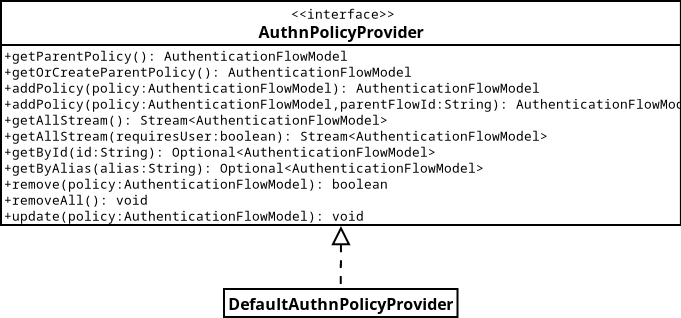
\includegraphics[width=1\textwidth]{img/sections/6-implementation/authn-policy-provider-diagram.png}
  \caption{Authentication Policy Provider}
  \label{fig:impl-authn-policies-provider-diagram}
\end{figure}

\newpage

The interface \textit{AuthnPolicyProvider} consists of the basic CRUD operations that can be made on authentication policies, such as:

\begin{itemize}
    \item \textit{getParentPolicy()} -- retrieve the parent \textit{Authentication policies - PARENT} flow.
    \item \textit{getOrCreateParentPolicy()} -- retrieve, or create if it does not exist, the parent \textit{Authentication policies - PARENT} flow.
    \item \textit{addPolicy(policy)} -- add a new policy \textit{policy} with the default parent flow.
    \item \textit{addPolicy(policy, parentFlowId)} -- add a new policy \textit{policy} with the parent flow \textit{parentFlowId}.
    \item \textit{getAllStream()} -- retrieve a stream of all authentication policies.
    \item \textit{getAllStream(requiresUser)} -- retrieve a stream of all authentication policies with the execution phase equal to \textit{requiresUser} attribute.
    \item \textit{getById(id)} -- retrieve an authentication policy found by provided ID via the \textit{id} attribute.
    \item \textit{getByAlias(alias)} -- retrieve an authentication policy found by provided alias via the \textit{alias} attribute.
    \item \textit{remove(policy)} -- remove a policy defined in the \textit{policy} attribute.
    \item \textit{removeAll()} -- remove all authentication policies.
    \item \textit{update(policy)} -- update an authentication policy provided via the \textit{policy} attribute.
\end{itemize}

\newpage
\subsubsection{Add Authentication Policy}
One of the most interesting examples of implementing methods of the \textit{AuthnPolicyProvider} interface is the \textit{addPolicy()} method shown in Figure \ref{fig:impl-authn-policies-add-policy-diagram}.
That method is responsible for creating a new authentication policy based on the parameters.

\begin{figure}[htbp]
  \centering
  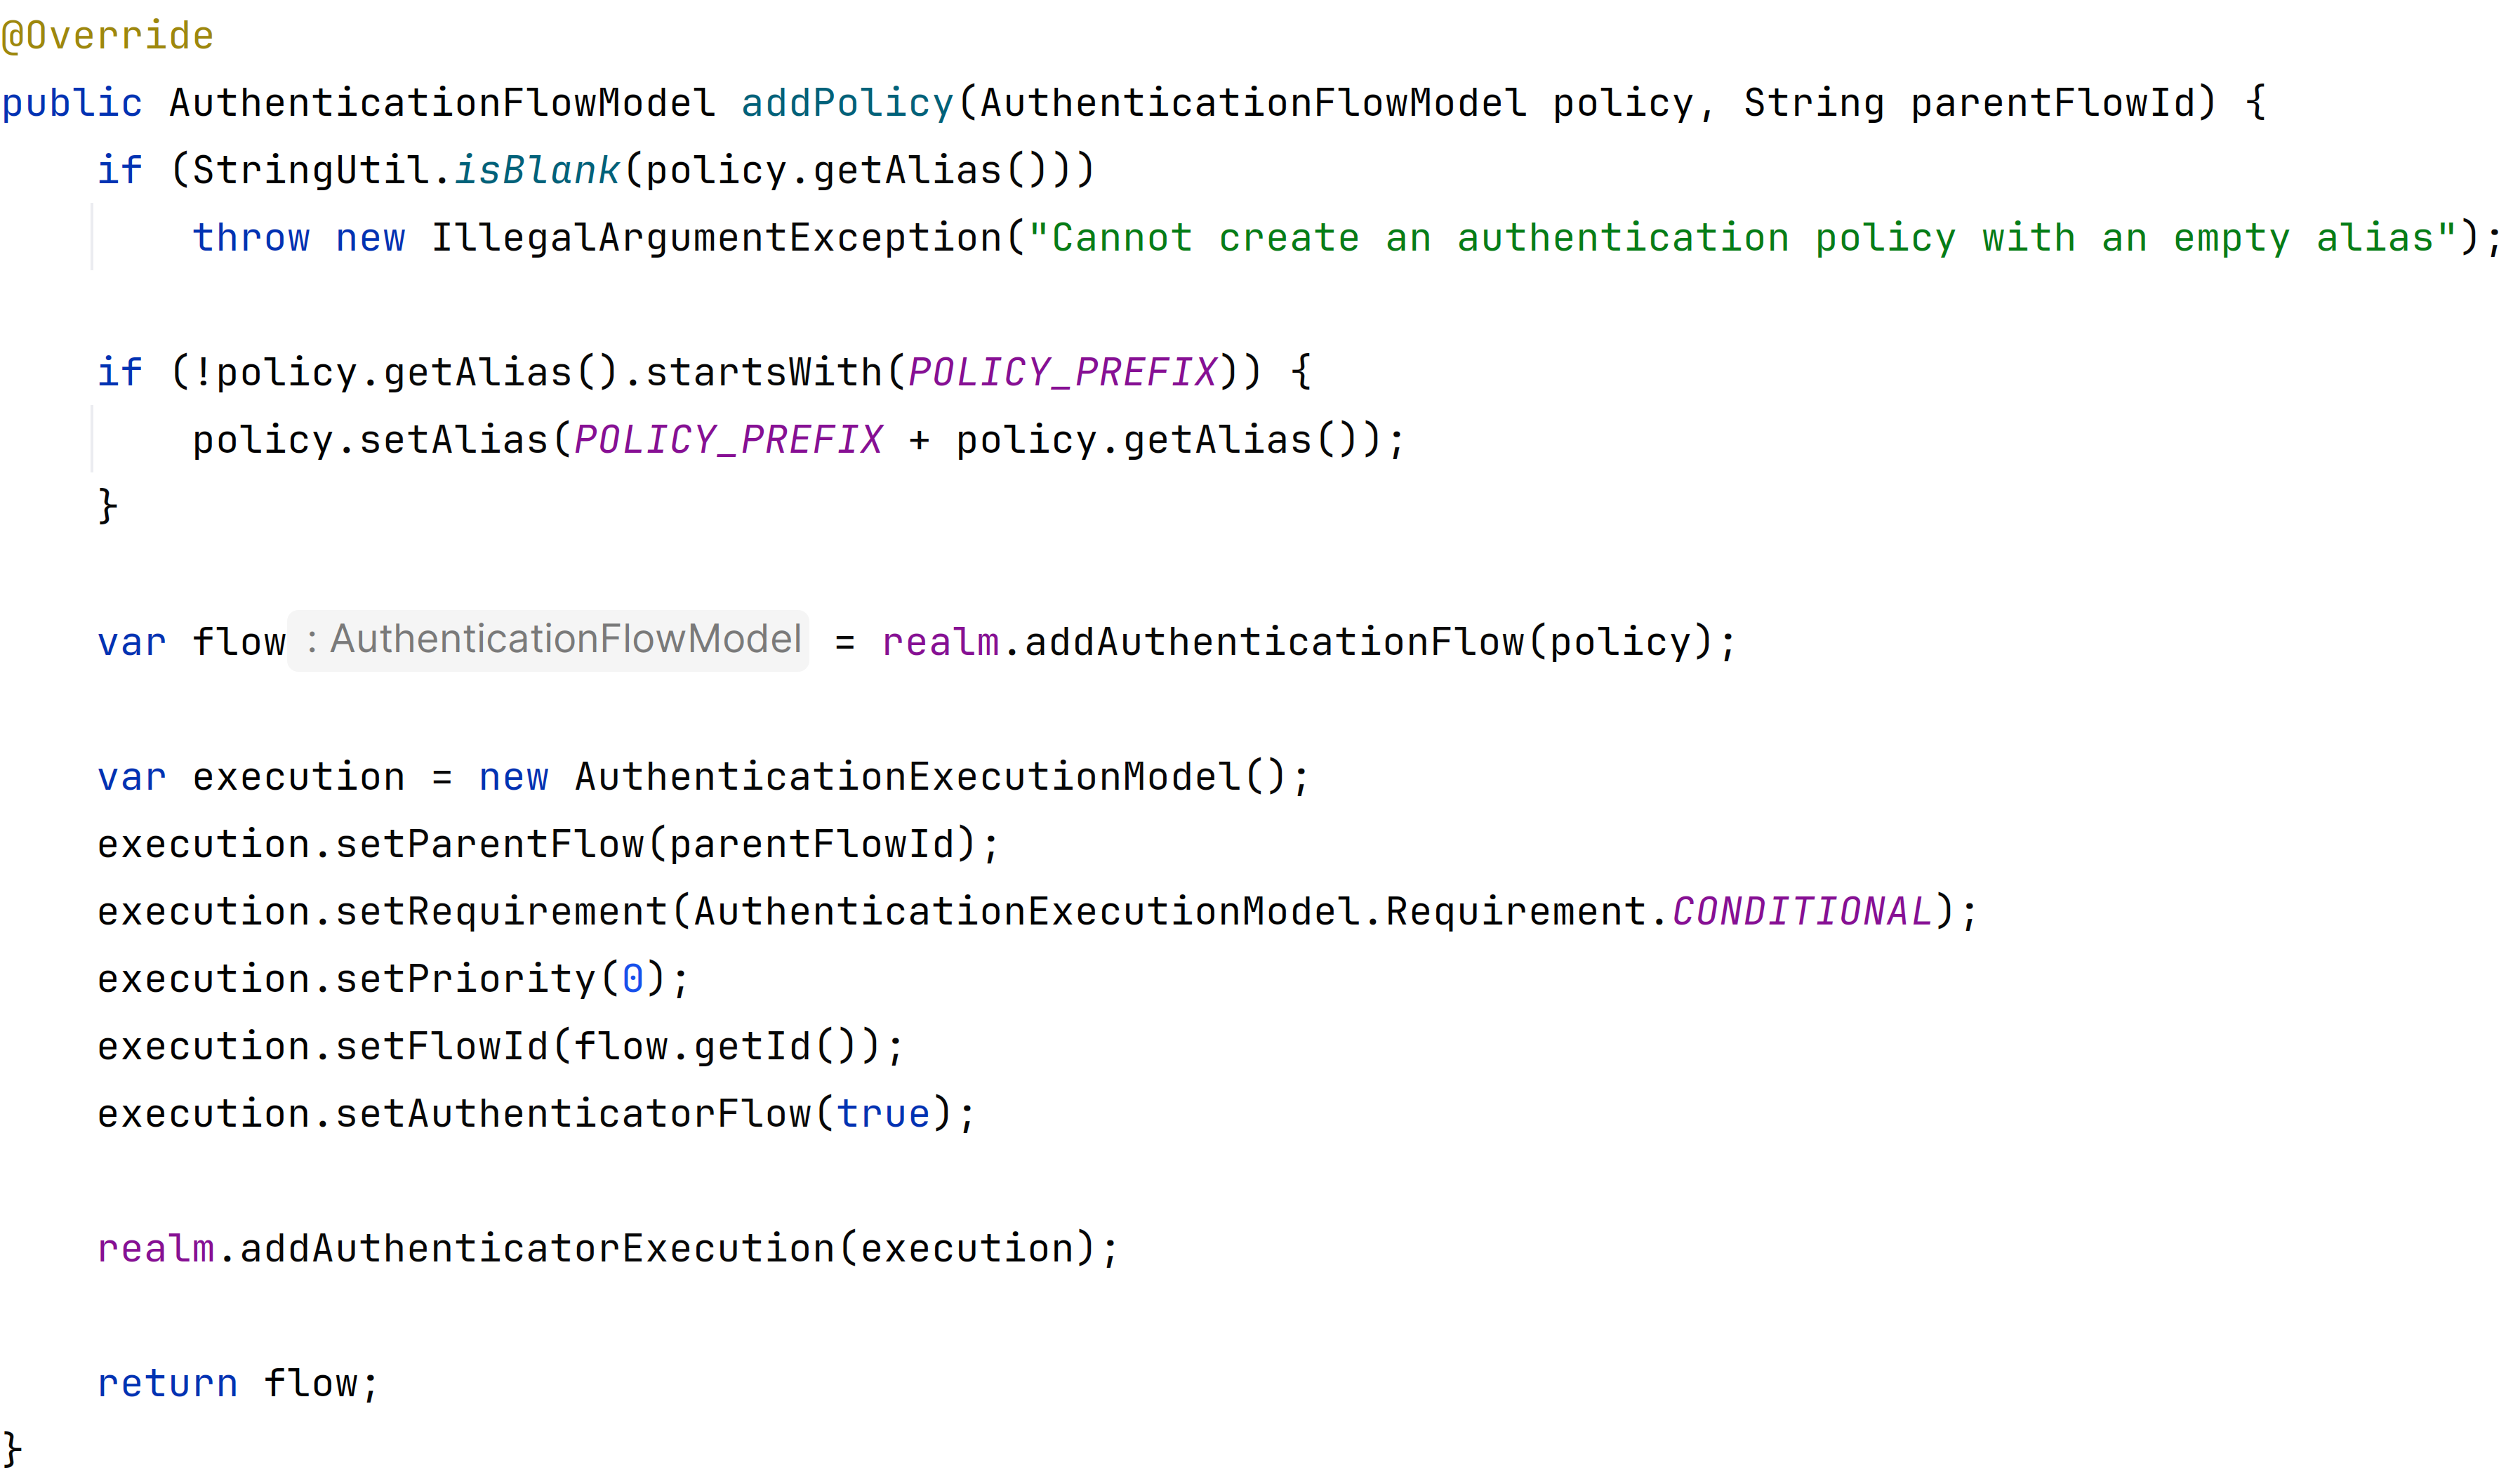
\includegraphics[width=1.05\textwidth]{img/sections/6-implementation/authnPolicyAddPolicy.png}
  \caption{Add Policy Method}
  \label{fig:impl-authn-policies-add-policy-diagram}
\end{figure}

First of all, the alias must not be empty.
Otherwise, the exception is thrown.
If the alias does not start with the prefix \textit{"POLICY - "}, it is automatically added to the alias.
The last part of the execution is to create a conditional flow where the parent flow is the common parent authentication flow for all authentication policies.
The newly created authentication policy is returned.

\newpage

\subsubsection{Retrieve Authentication Policies}

Another method worth mentioning is the \textit{getAllStream(requiresUser)}, shown in Figure \ref{fig:impl-authn-policies-get-all}.
The method returns all authentication policies that match the \textit{requiresUser} boolean attribute.
Specifically, it iterates over all policies, and if there is some requirement to require a user, it automatically includes it in the final stream.
It does not consider several layers of authentication policies hierarchy.
If the execution authenticator implements the \textit{ConfigurableRequirements} interface, the condition of whether it requires a user is evaluated dynamically.

\begin{figure}[htbp]
  \centering
  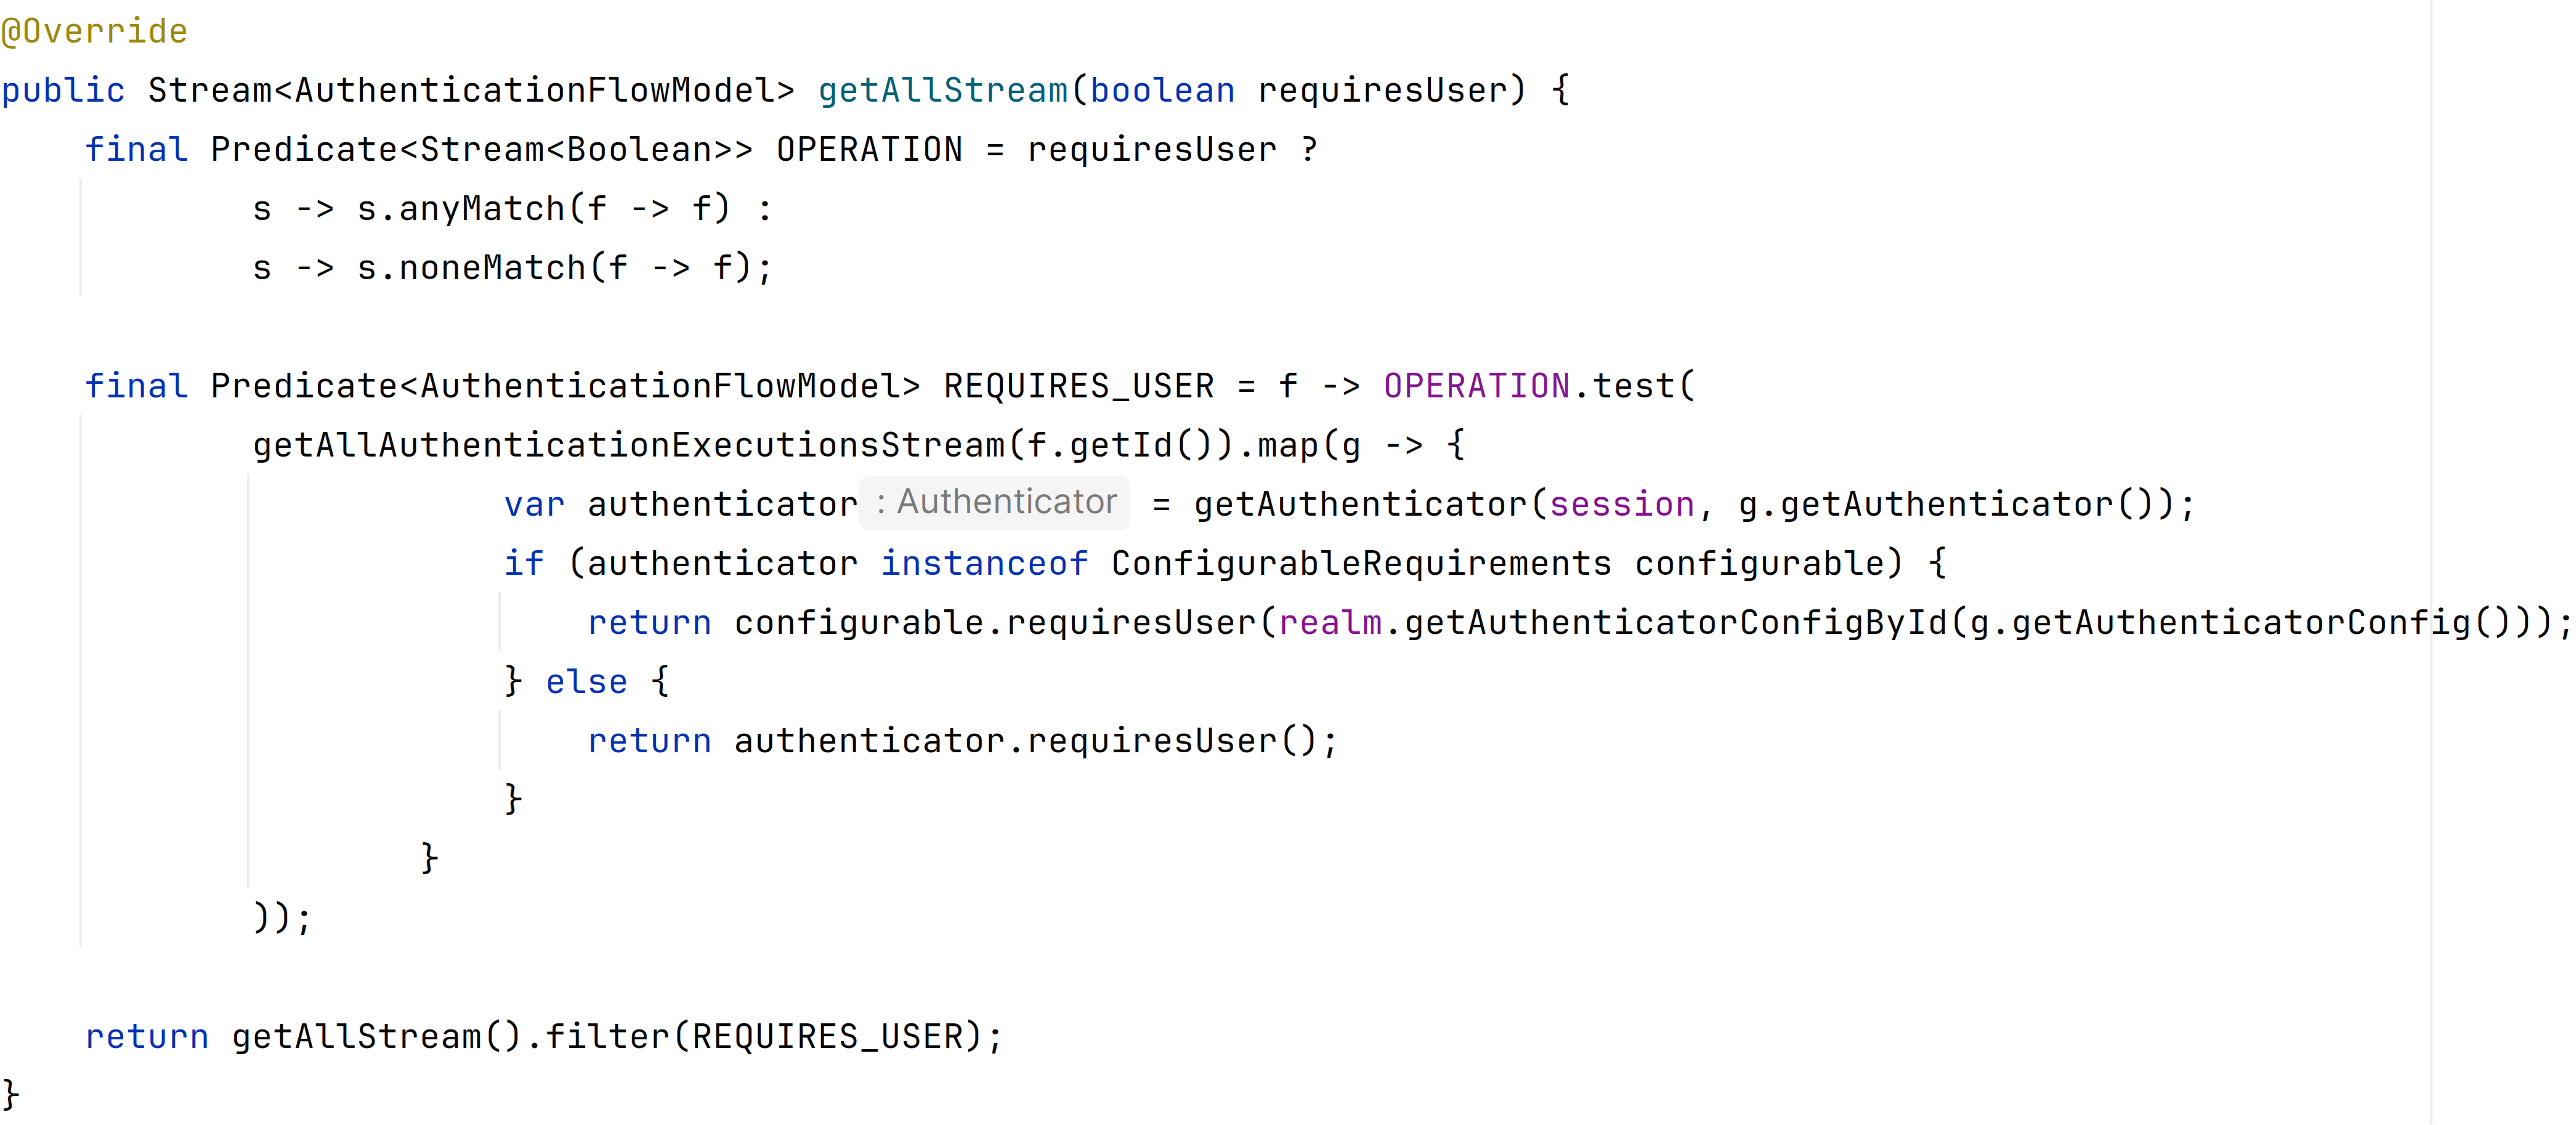
\includegraphics[width=1\textwidth]{img/sections/6-implementation/authnPolicyGetAllStream.png}
  \caption{Get All Authentication Policies}
  \label{fig:impl-authn-policies-get-all}
\end{figure}

The helper method \textit{getAllAuthenticationExecutionsStream} shown in Figure \ref{fig:impl-authn-policies-get-all-execs} returns all executions included in the authentication policy with the usage of recursion.

\begin{figure}[htbp]
  \centering
  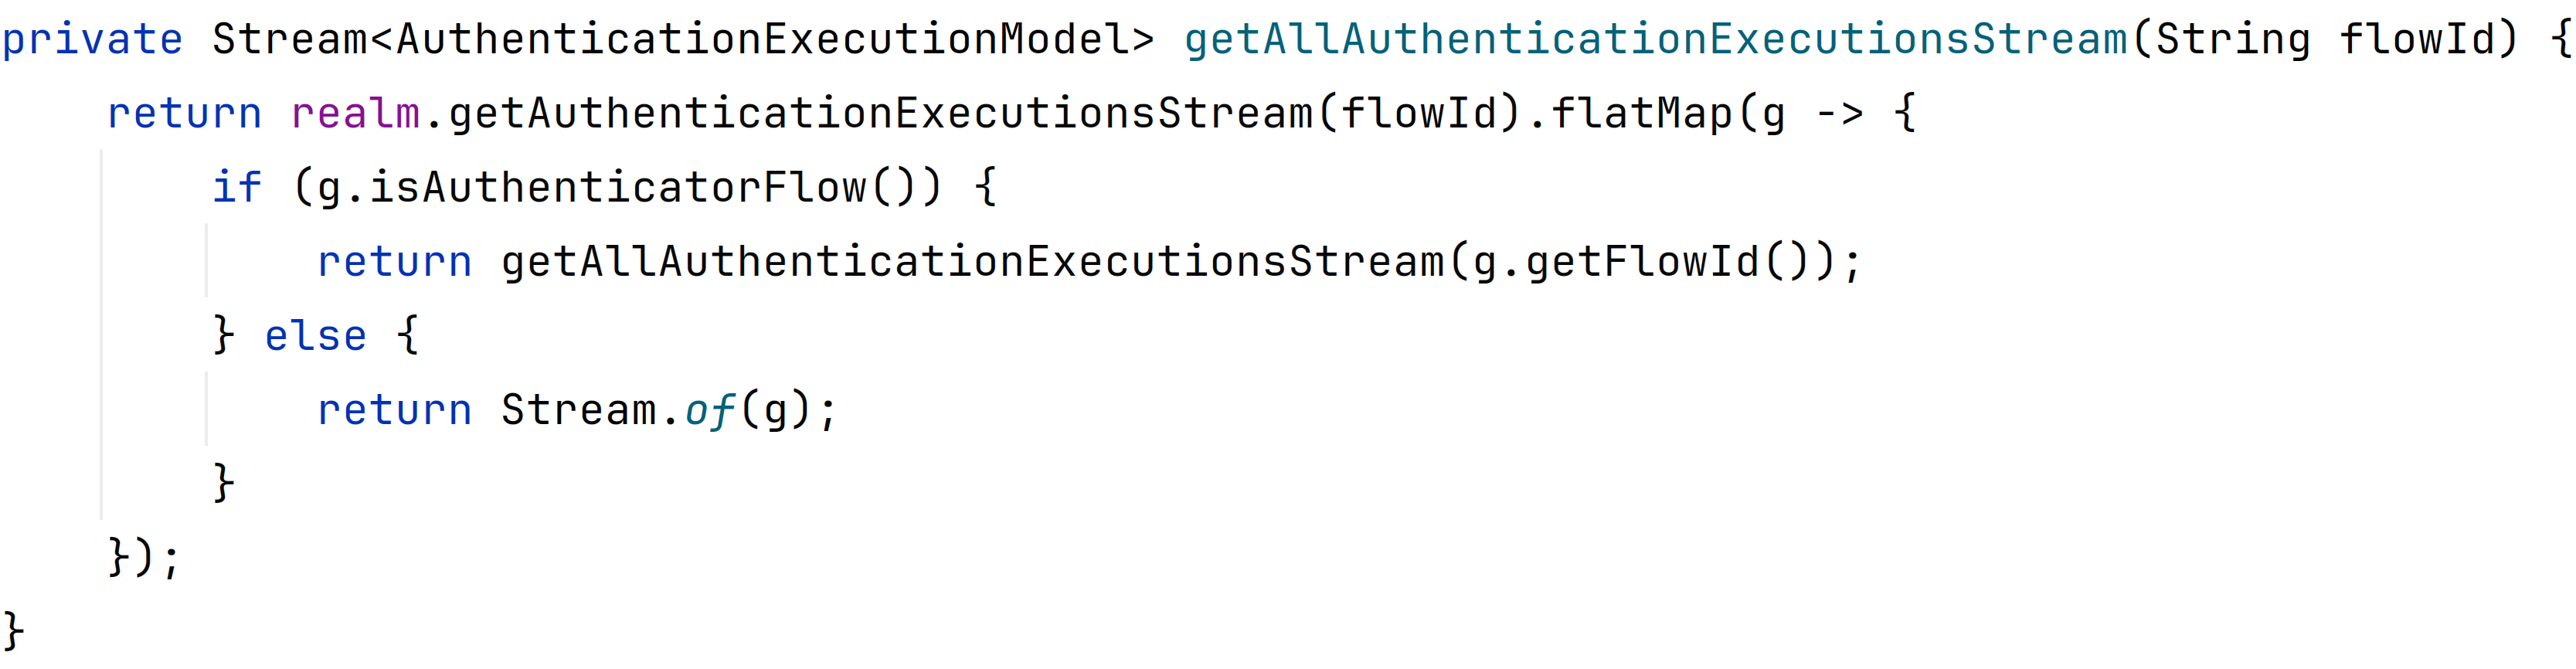
\includegraphics[width=0.95\textwidth]{img/sections/6-implementation/authnPolicyGetAllExecutions.png}
  \caption{Get All Authentication Executions}
  \label{fig:impl-authn-policies-get-all-execs}
\end{figure}

\newpage
\subsection{REST API} \label{impl-authn-policies-rest}
A REST API (also known as RESTful API) is an API that conforms to the constraints of REST architectural style and allows for interaction with RESTful web services.
REST stands for \textit{REpresentational State Transfer}.\cite{impl-rest} 

A client accessing the REST API through the parent endpoint \textit{/authn-policies} defined for the \textit{AuthnPoliciesResource} request handler class.
When an HTTP request is sent to the endpoint, it is handled by the class, which directs it to the appropriate method based on the HTTP method of the request, shown in Figure \ref{fig:impl-authn-policies-rest}.

The request handler classes work explicitly with the authentication policy DAO, described in Section \ref{impl-authn-policies-dao}.
It provides the isolation of storage operations and user interaction and complies with the Single-responsibility principle.\cite{impl-single-responsibility}

\begin{figure}[htbp]
  \centering
  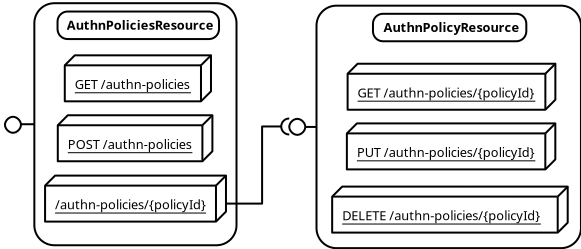
\includegraphics[width=0.9\textwidth]{img/sections/6-implementation/rest.png}
  \caption{Authentication Policies REST API}
  \label{fig:impl-authn-policies-rest}
\end{figure}

Possible operations on the \textit{AuthnPoliciesResource} request handler class with the additional redirection:
\begin{itemize}
    \item \textit{GET /authn-policies} -- retrieve all authentication policies in JSON format. 
    \item \textit{POST /authn-policies} -- create a new authentication policy with attributes defined as JSON in the request body.  
    \item \textit{/authn-policies/{policyId}} -- Redirects requests to the \textit{AuthnPolicyResource} request handler class.
\end{itemize}

Possible operations on the \textit{AuthnPolicyResource} request handler class:

\begin{itemize}
    \item \textit{GET /authn-policies/\{policyId\}} -- retrieve an authentication policy with ID \textit{policyId} in JSON format.
    \item \textit{PUT /authn-policies/\{policyId\}} -- update an existing authentication policy with ID \textit{policyId} with attributes defined as JSON in the request body.
    \item \textit{DELETE /authn-policies/\{policyId\}} -- delete an existing authentication policy with ID \textit{policyId}.
\end{itemize}

The exact implementation of a specific part of the \textit{AuthnPoliciesResource} class is shown in Figure \ref{fig:impl-authn-policies-rest-impl}.
In the constructor, all necessary initializations are done, and the authentication policy DAO is injected.
When the HTTP request with the \textit{GET} request method is sent to the endpoint, the \textit{getPolicies()} method returns the set of policies in a serialized JSON format.
The abstract model representation is converted to the \textit{Data Transfer Object} (DTO) and returned to the client.

\begin{figure}[htbp]
  \centering
  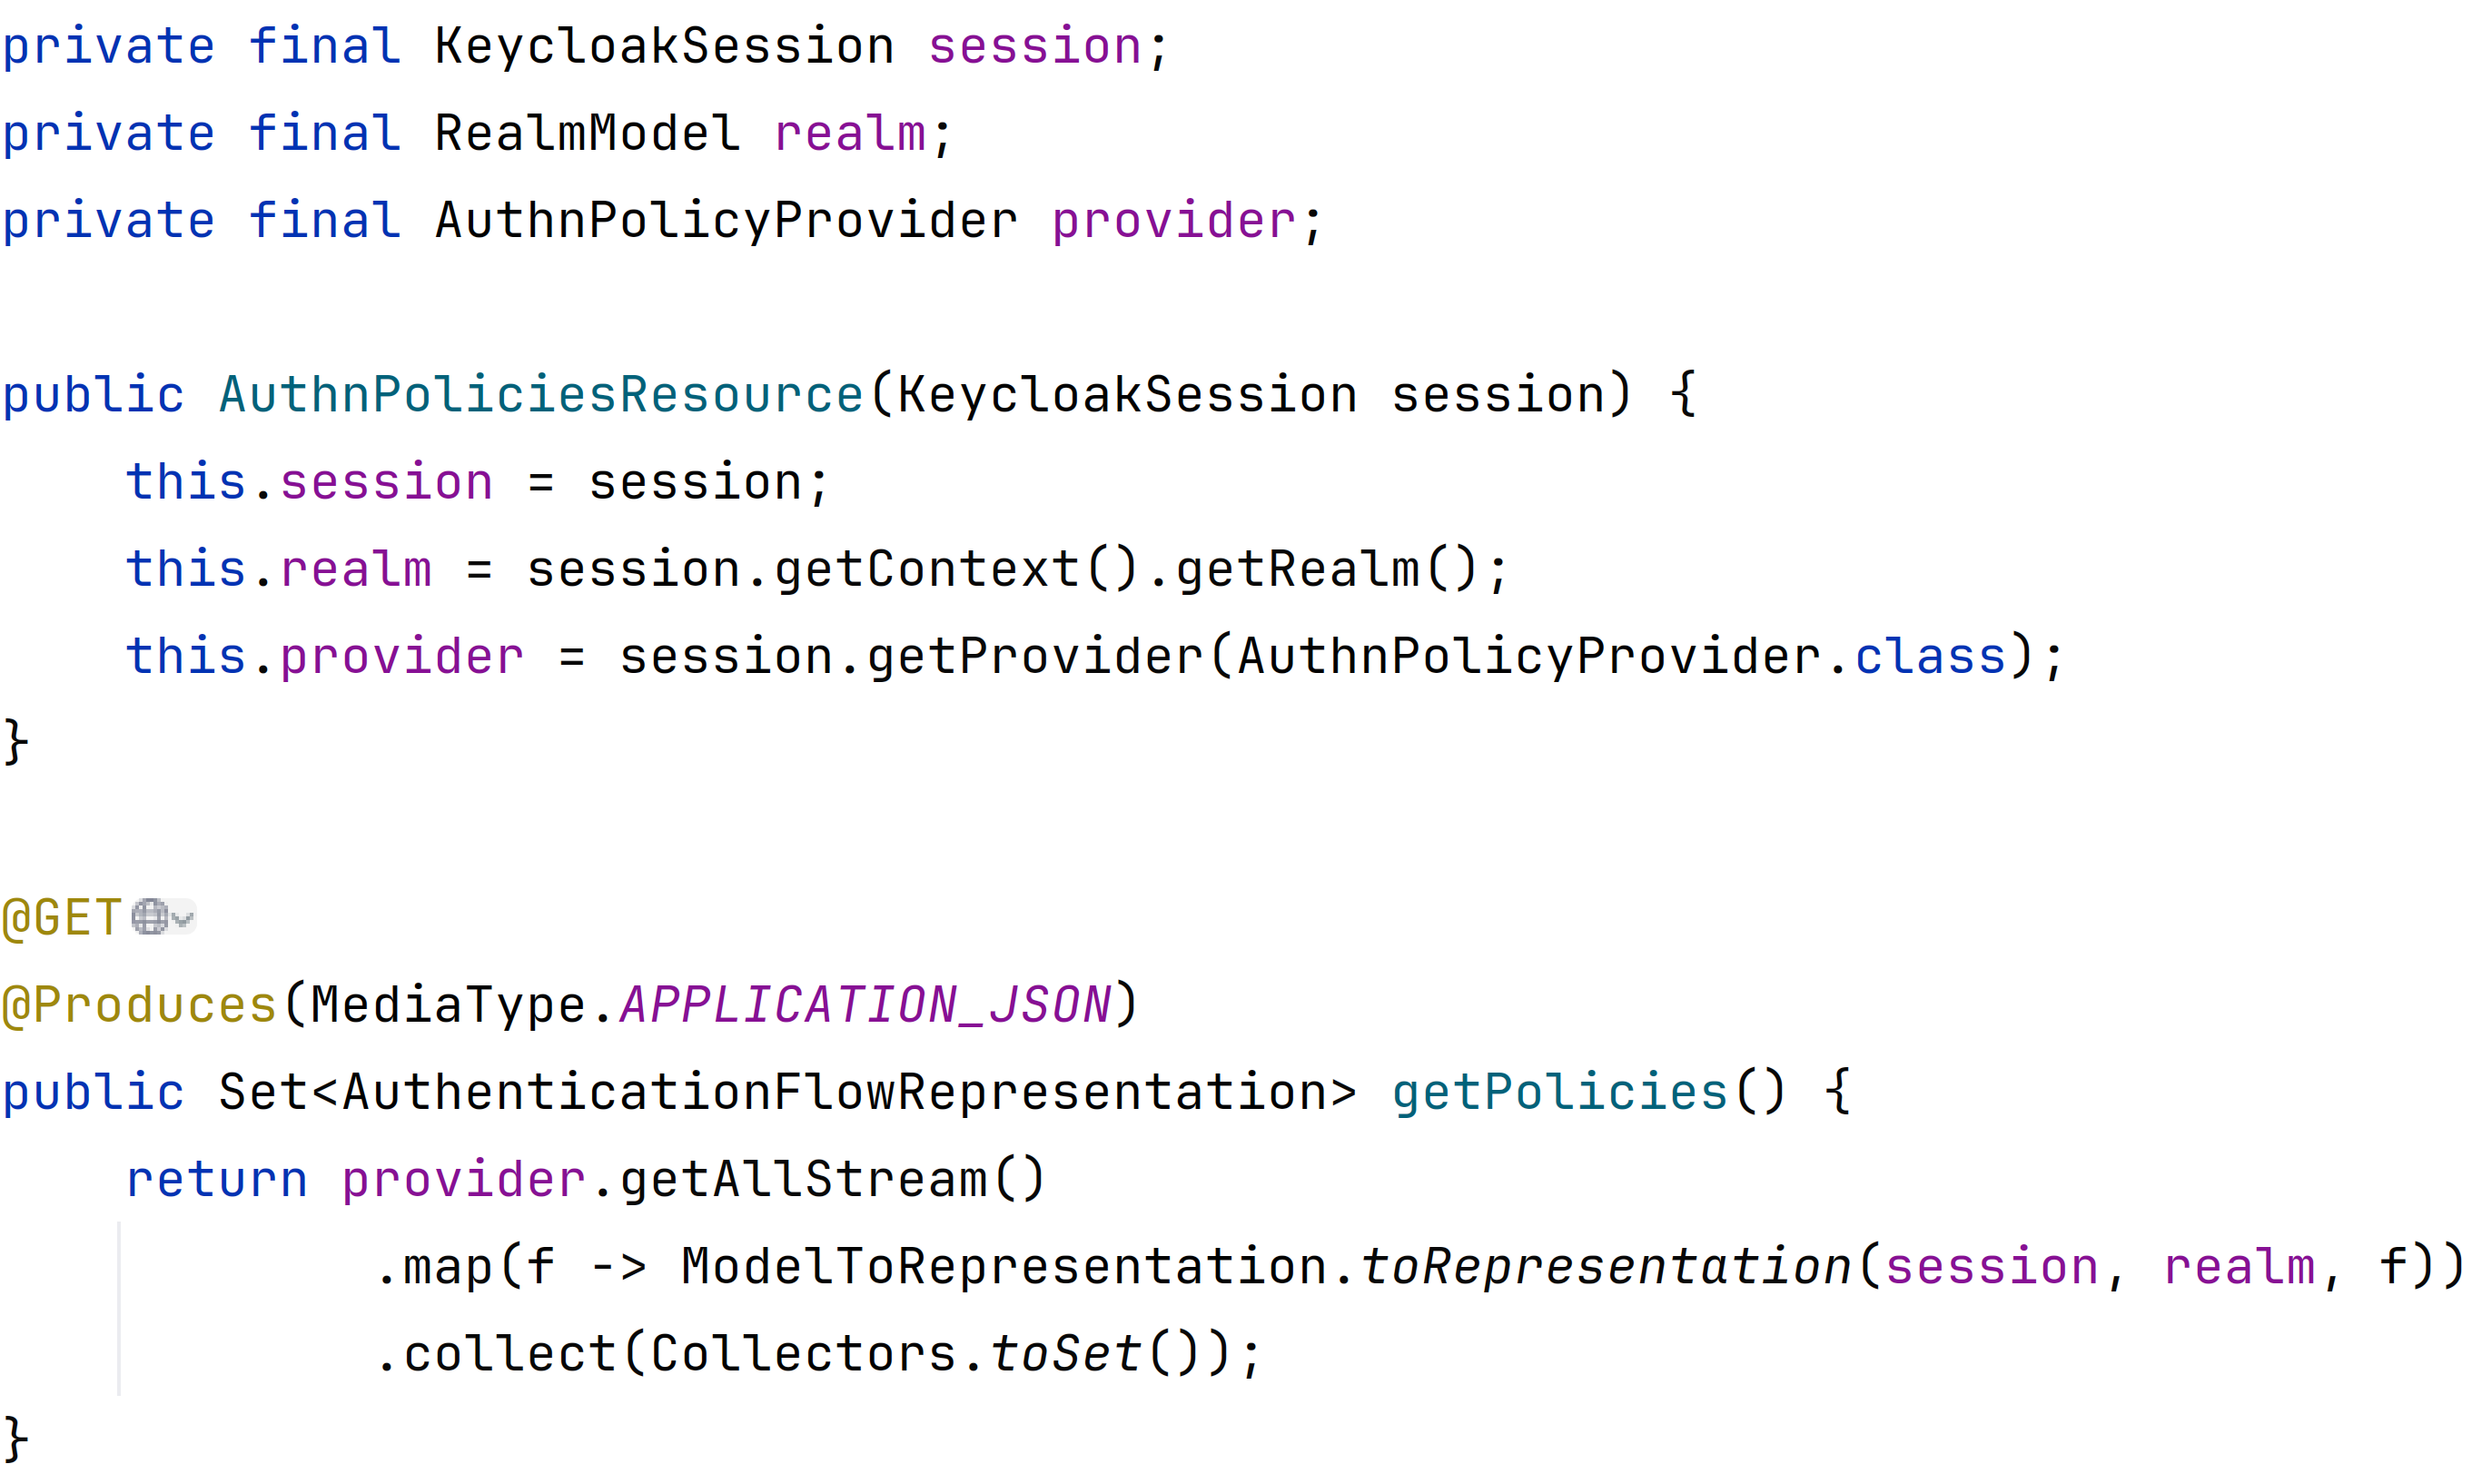
\includegraphics[width=1\textwidth]{img/sections/6-implementation/authn-policy-rest-example.png}
  \caption{Authentication Policies REST API Implementation}
  \label{fig:impl-authn-policies-rest-impl}
\end{figure}

\newpage

\subsection{Administrator Console} \label{impl-authn-policies-admin}

\newpage
\section{User Context}
The first step for implementing the \textit{UserContext<T>} interface is to bind the generic type to the required one, either through extending the interface or directly in the implementation of the context.

For demonstration purposes, consider a specific user context \textit{IpProxyContext}, which handles all IP addresses present in the HTTP \textit{Forwarded}, and \textit{X-Forwarded-For} headers used when a proxy is part of the deployment.

The specific \textit{IpProxyContext} was created, shown in Figure \ref{fig:impl-user-ctx-ifc}, in order to bind the type of the user context with a possible extension of it.

\begin{figure}[htbp]
  \centering
  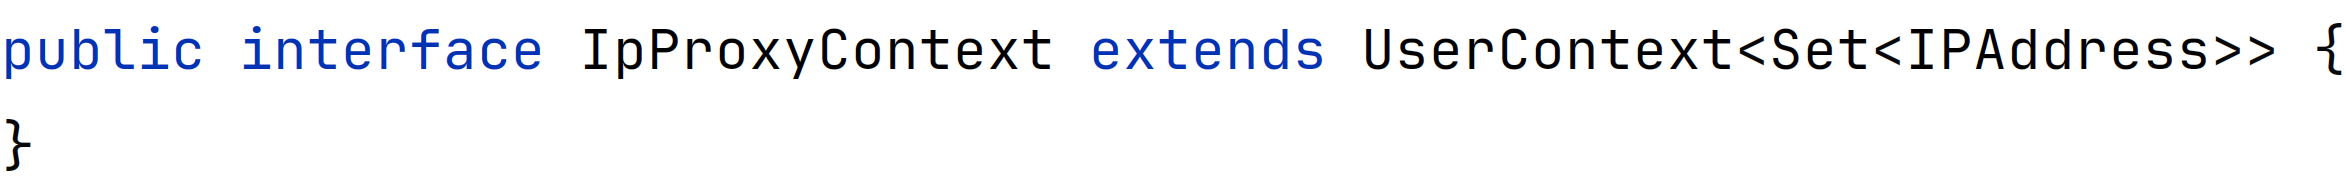
\includegraphics[width=1\textwidth]{img/sections/6-implementation/proxyIpAddressContextInterface.png}
  \caption{Extend \textit{UserContext} Interface}
  \label{fig:impl-user-ctx-ifc}
\end{figure}

The implementation of the \textit{IpProxyContext}, shown in Figure \ref{fig:impl-user-ctx-ip}, consists of several attributes to fulfill the requirements of the interface by returning particular data in methods.

In the constructor, the \textit{initData()} method is called, which initializes data when the context is needed.
With the help of the \textit{KeycloakSession}, the data for a particular context is processed only once per request, so when different risk evaluators need the context, it is not evaluated multiple times.

During the initialization of the data, the HTTP headers of the current request are parsed.
IP addresses included in the headers \textit{Forwarded} and \textit{X-Forwarded-For} are concatenated together.
When there is valid data, the boolean flag \textit{isInitialized} is set to \textit{true}, which notes the initialization is done correctly and data is available. 

\begin{figure}[htbp]
  \centering
  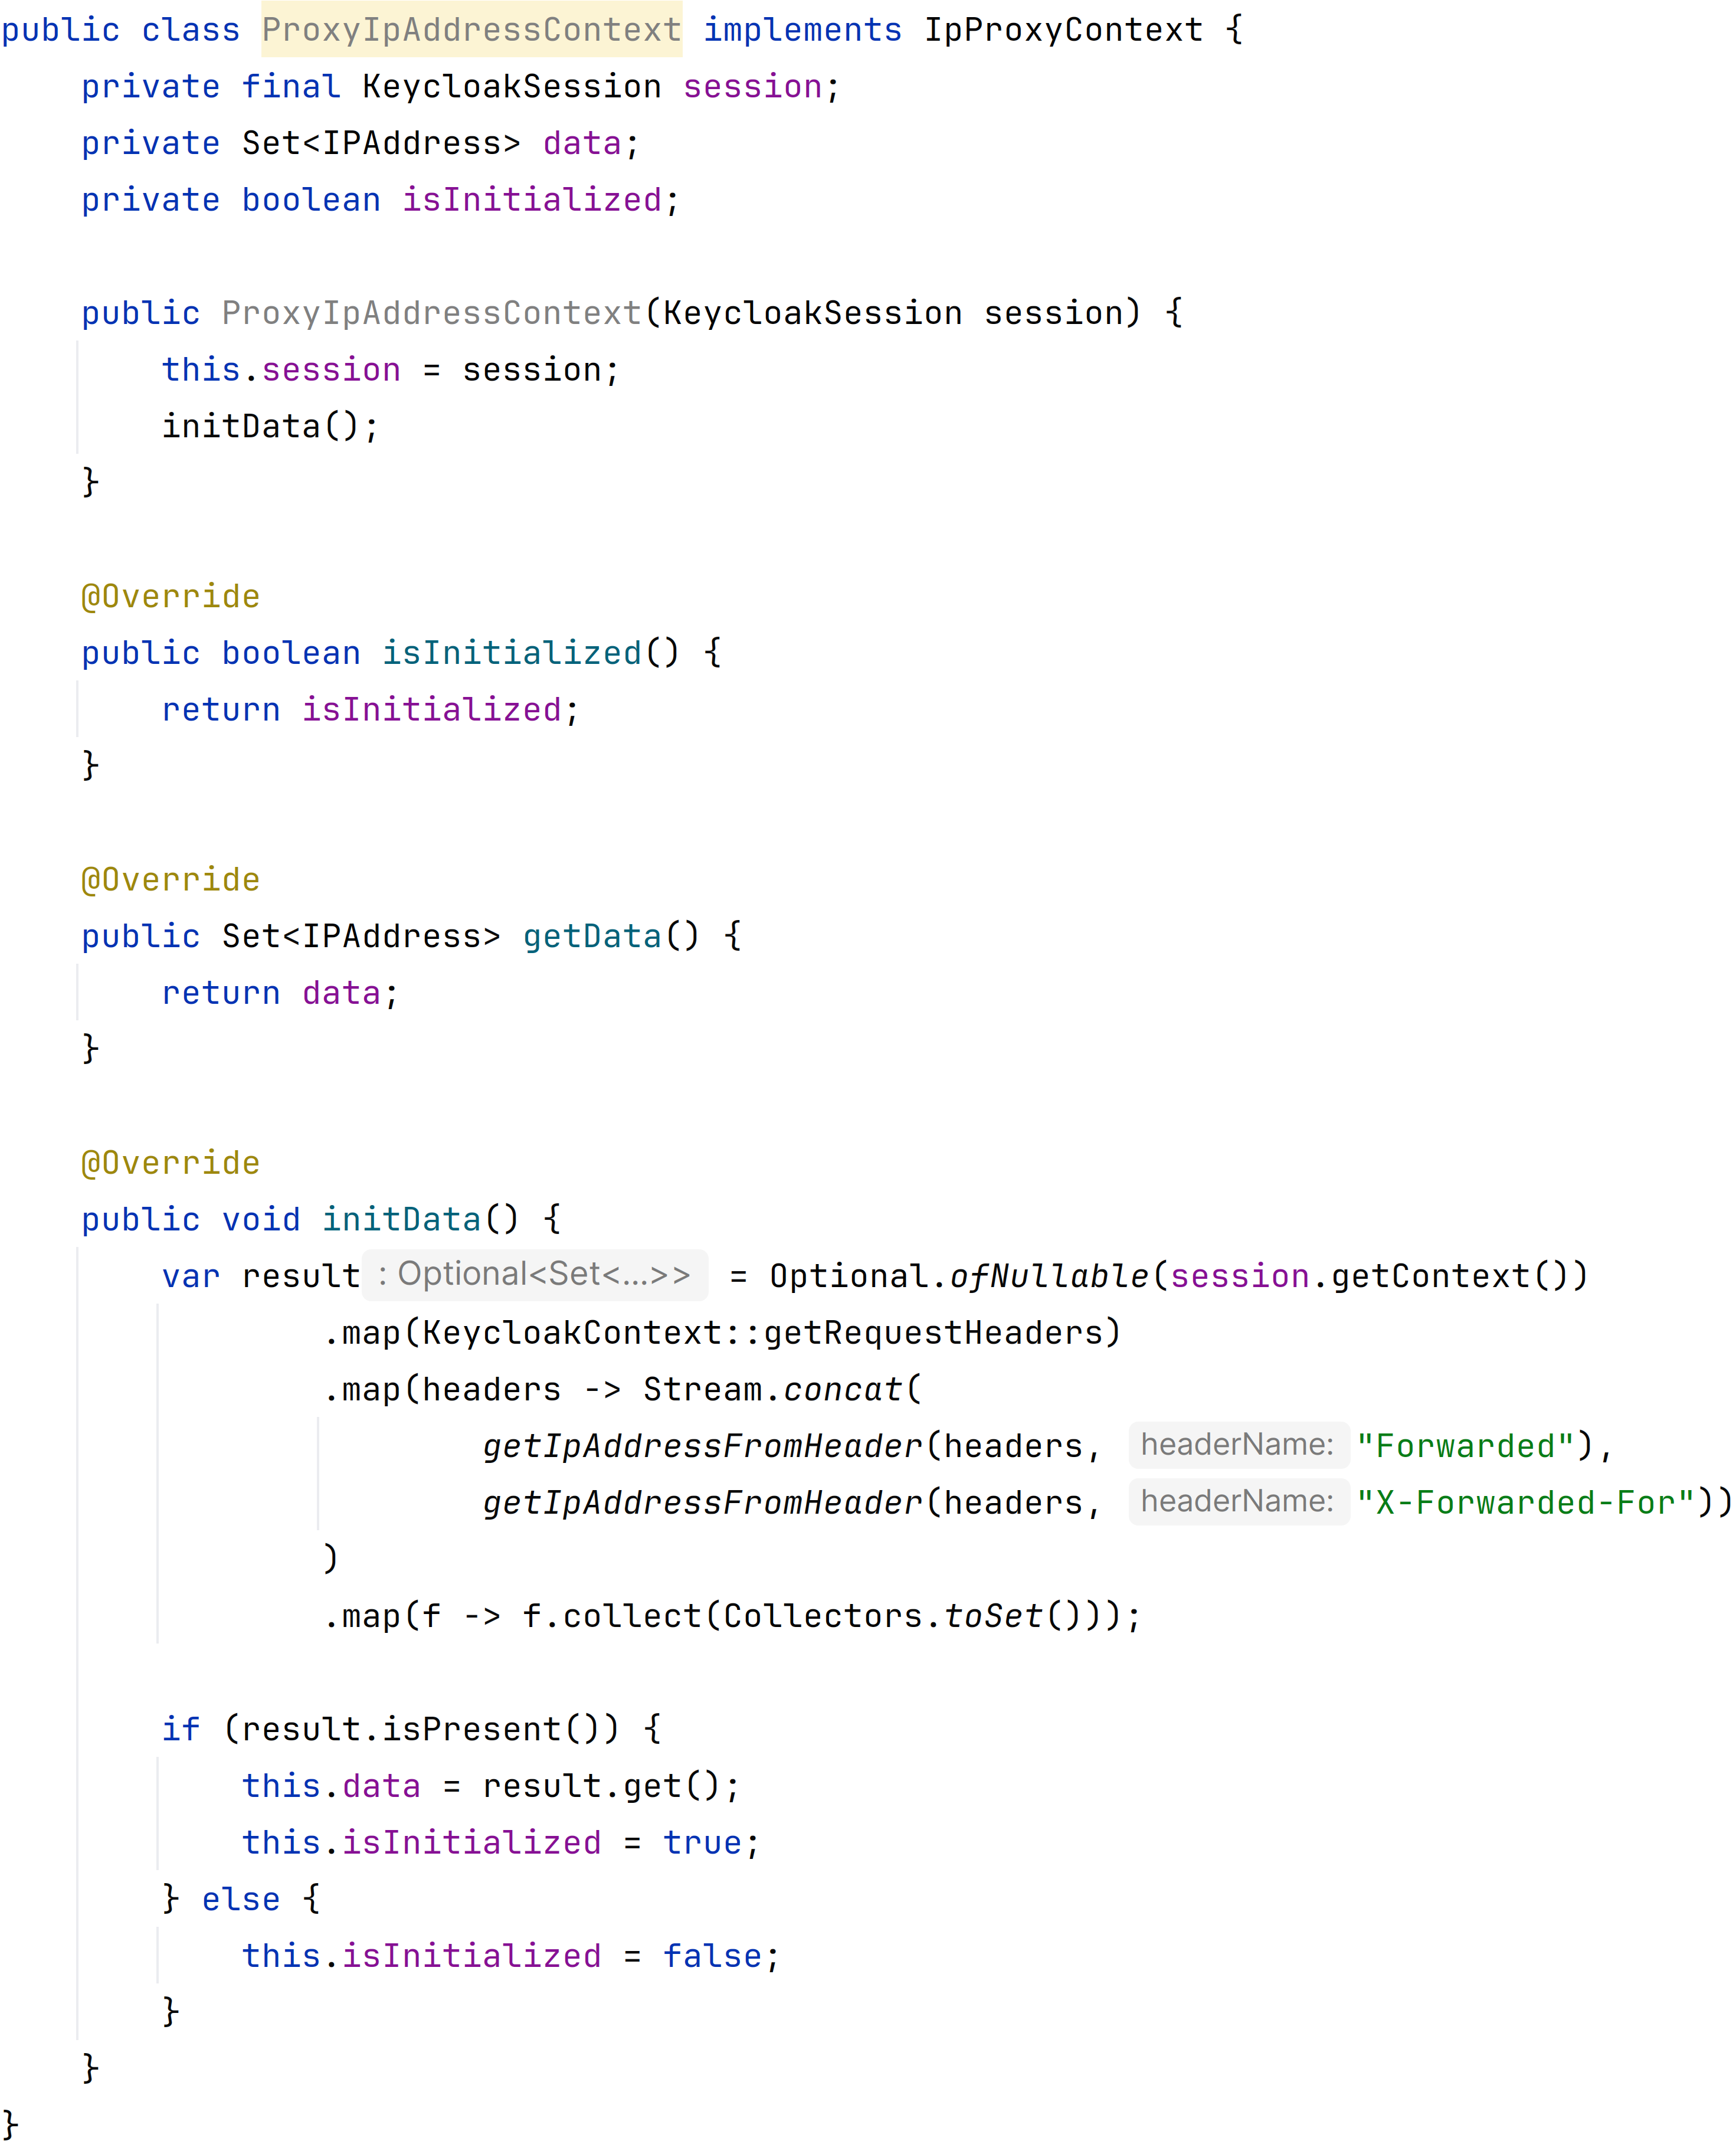
\includegraphics[width=1\textwidth]{img/sections/6-implementation/proxyIpAddress-full.png}
  \caption{Implementation of the \textit{IpProxyContext}}
  \label{fig:impl-user-ctx-ip}
\end{figure}

\newpage
\section{Risk Evaluator}
A suitable example for the risk evaluator implementation is the specific \textit{LoginFailuresRiskEvaluator}, which statically evaluates the risk based on login failures shown in Figure \ref{fig:impl-risk-evaluator-login-failures}.
For further evaluation, the current IP address is required, so it is obtained from the \textit{IpAddressContext}.

The evaluated risk is returned as \textit{Optional}, as the risk might not be evaluated in time or at all. 
It helps to avoid working with \textit{null} values.
This evaluator requires to have information about the authentication user, so the method \textit{requiresUser()} is amended based on it.

\begin{figure}[htbp]
  \centering
  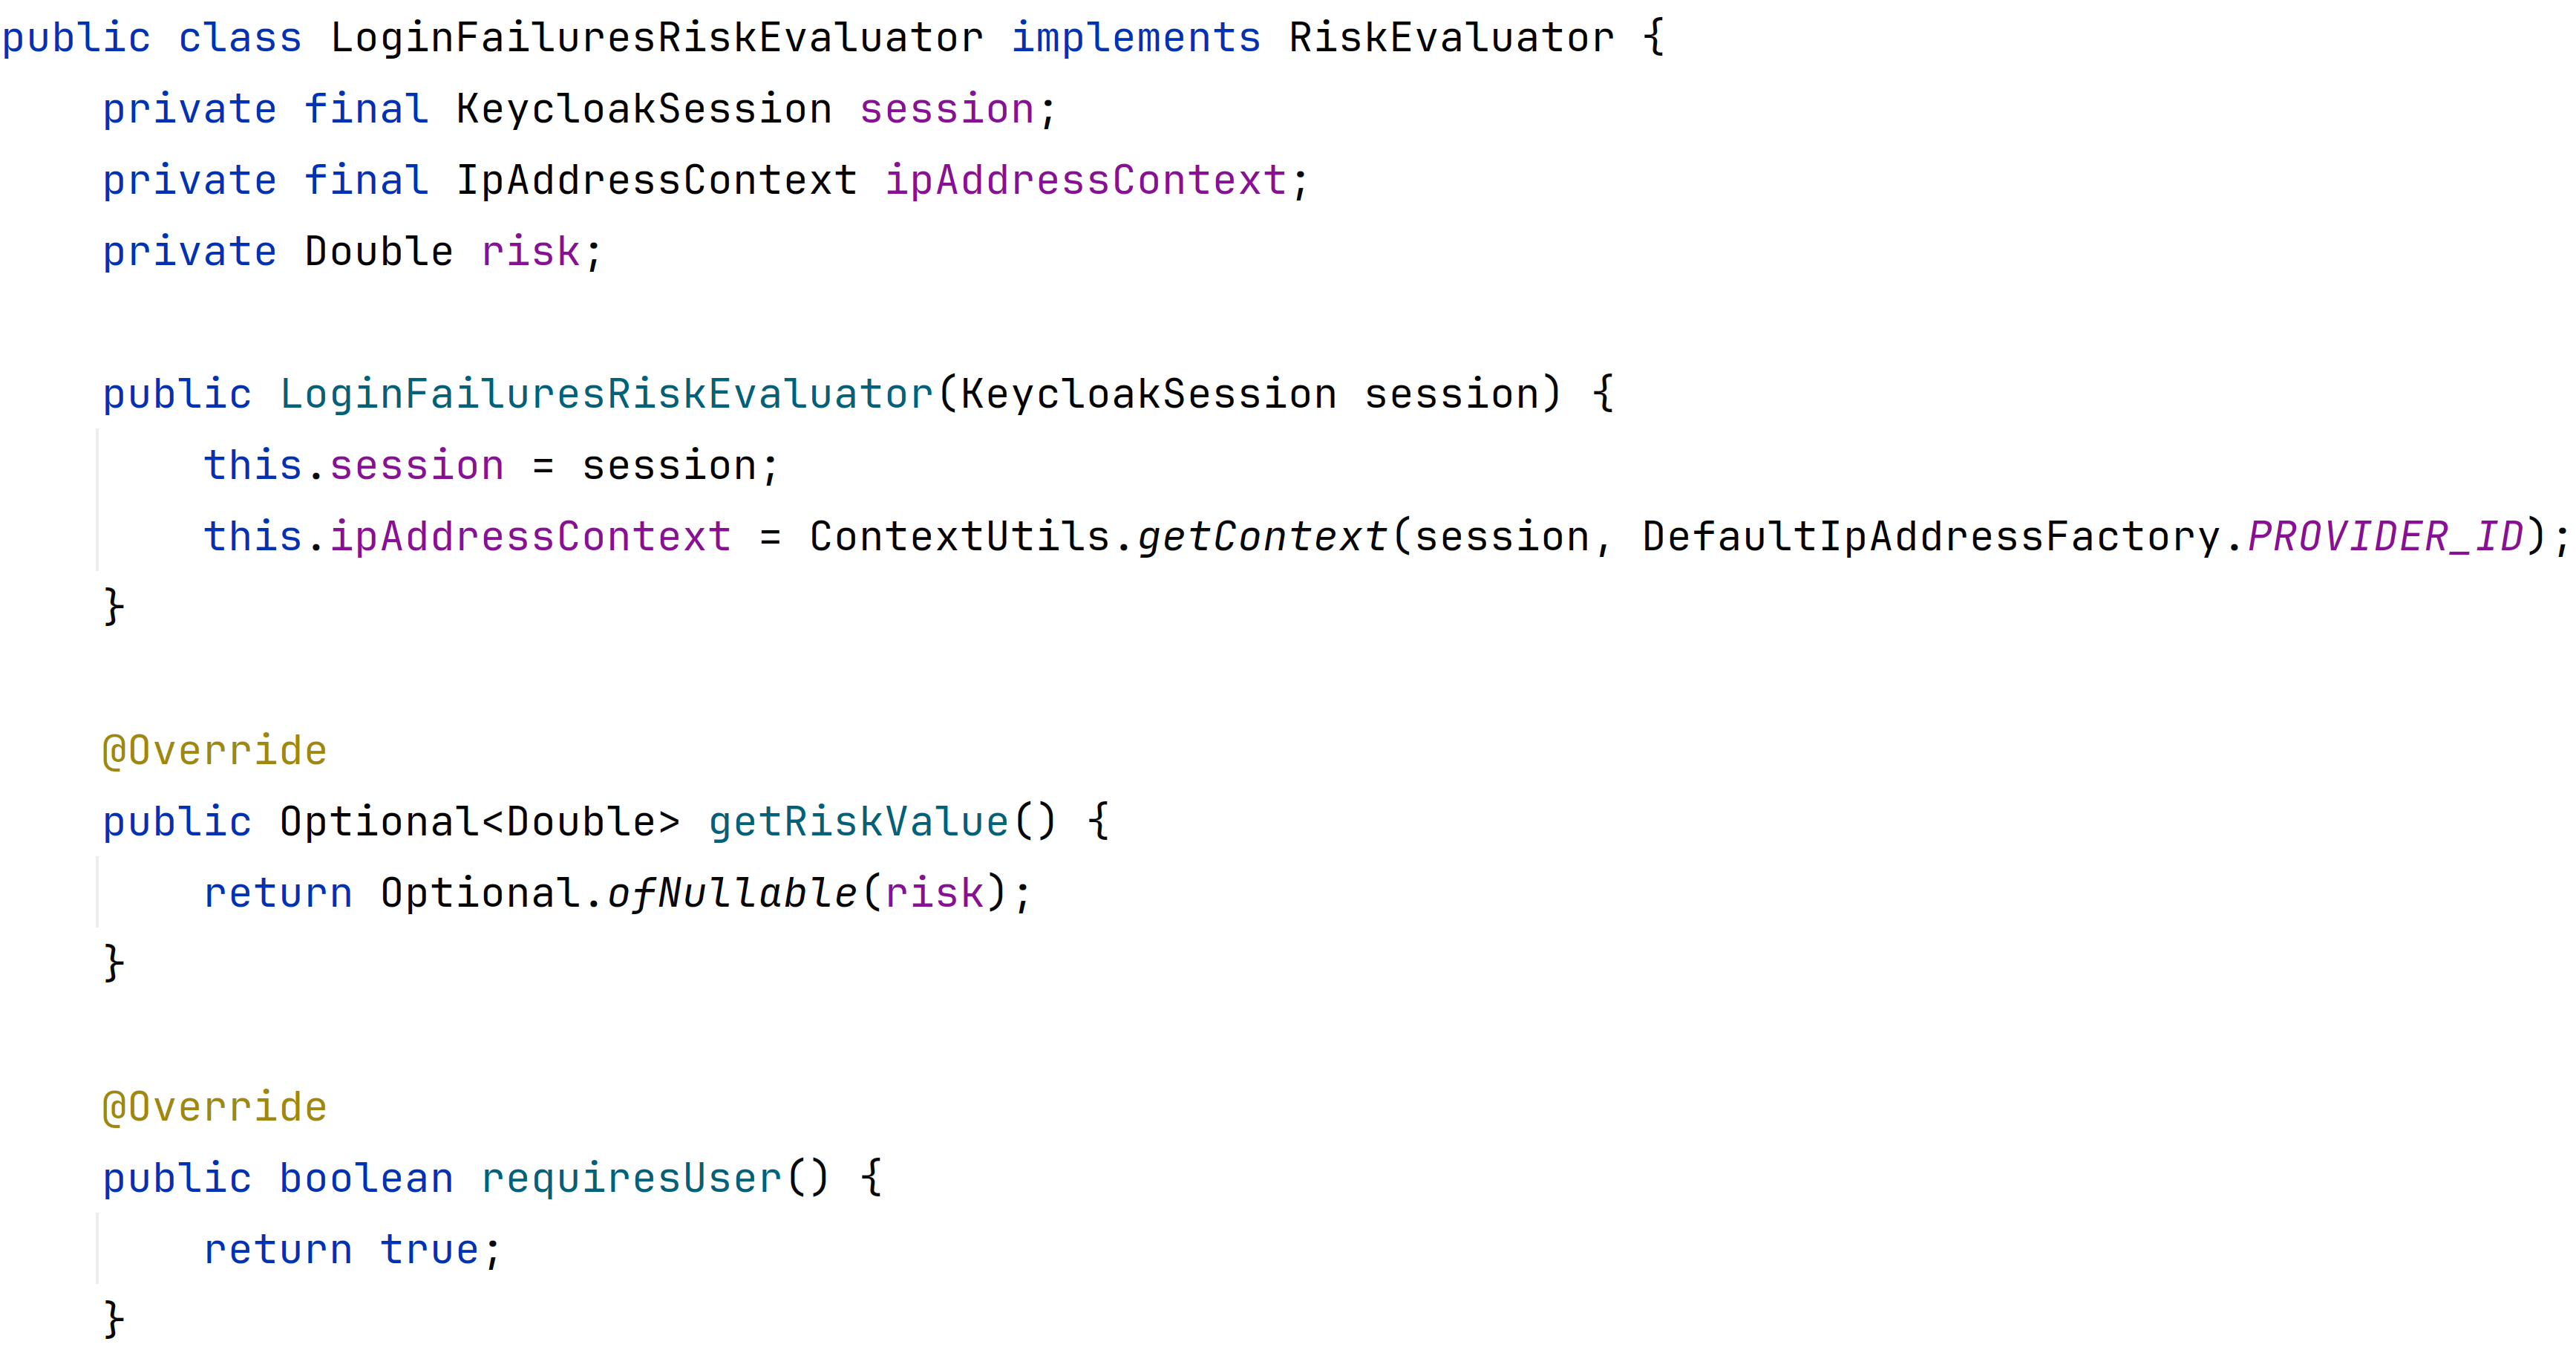
\includegraphics[width=1\textwidth]{img/sections/6-implementation/loginFailures.png}
  \caption{Login Failures Risk Evaluator}
  \label{fig:impl-risk-evaluator-login-failures}
\end{figure}

The evaluation of the risk itself is done in the \textit{evaluateRisk()} method, which contains a few checks of login failures, as shown in Figure \ref{fig:impl-risk-evaluator-login-failures-evaluations}.
As was mentioned before, the evaluation of the risk itself might be challenging and requires specific agreements on the evaluations, as there is no explicit correct approach to achieving it.

In the example, the risk is increasing based on the count of login failures, which might represent a brute-force attack.
The higher the count of login failures, the higher the risk.

\newpage
The last check verifies the current IP address and the IP address of the last login failure, as requesting resources from different IP addresses should indicate a higher risk.
There might be a situation where the risk for a legitimate user trying to access the application will be higher, as some fraudulent activity has been executed based on their account. 

\begin{figure}[htbp]
  \centering
  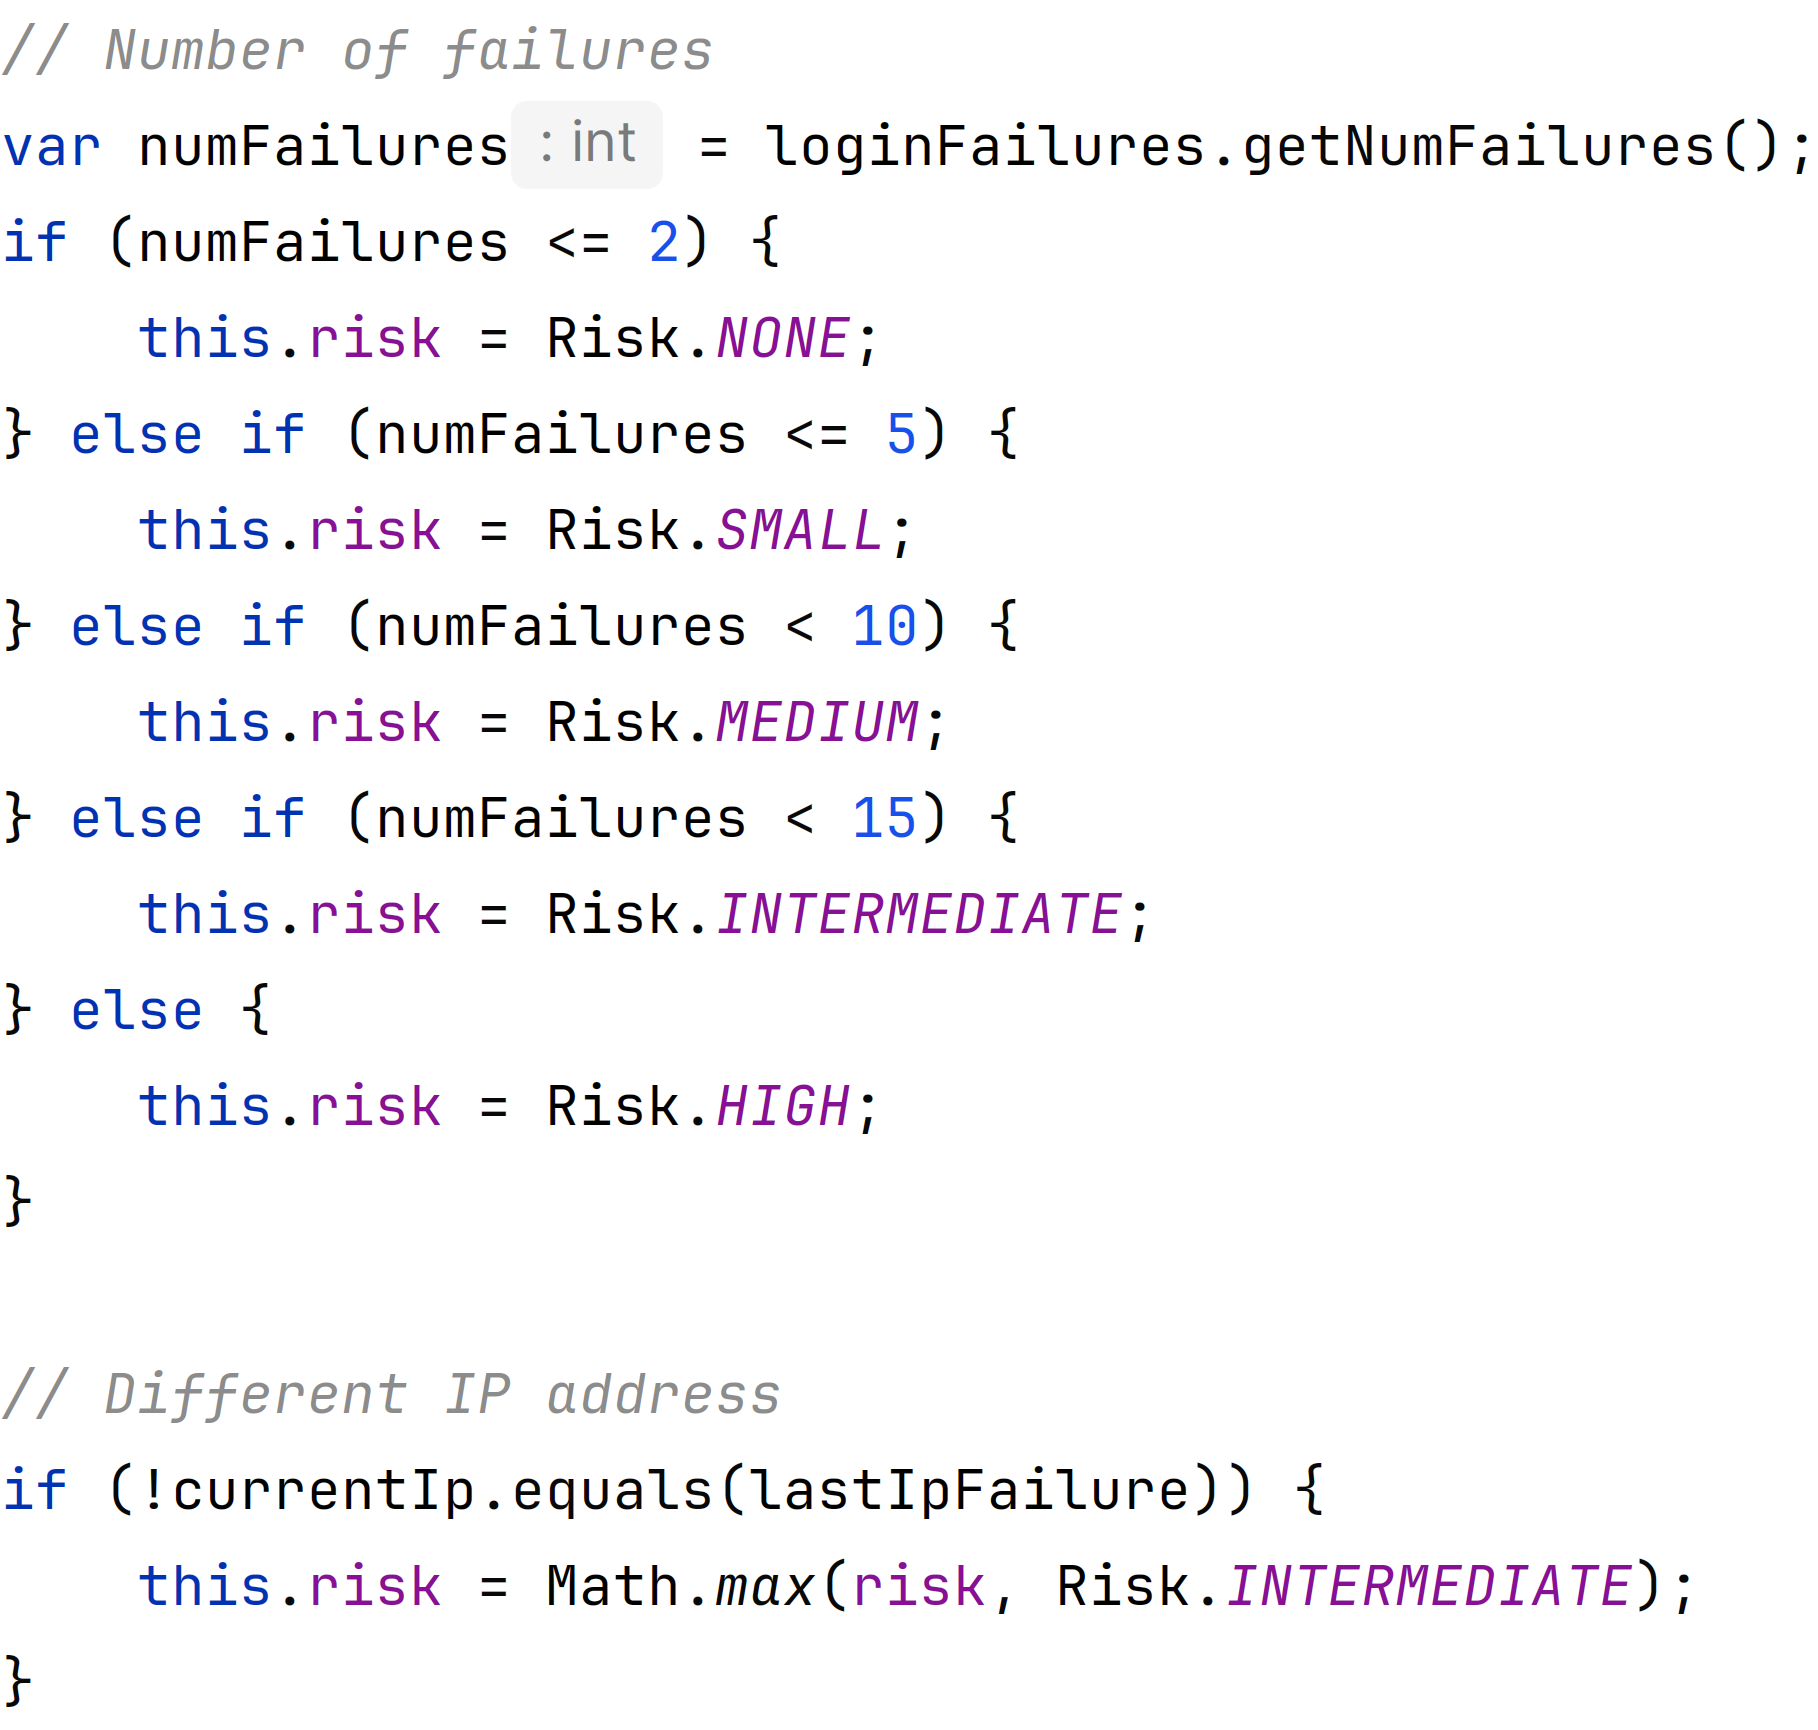
\includegraphics[width=0.7\textwidth]{img/sections/6-implementation/loginFailuresEvals.png}
  \caption{Login Failures Risk Evaluator Evaluations}
  \label{fig:impl-risk-evaluator-login-failures-evaluations}
\end{figure}

\newpage
\subsection{Configuration}
By default, for every risk evaluator, attributes \textit{isEnabled} and \textit{weight} can be configured by the administrator, as described in Section \ref{design-risk-eval-config}.
The permanent storing of the configuration of risk evaluators is done via realm attributes, which are represented by a key-value map structure.
Every configurable attribute of the risk evaluator has a unique key that is used to reference it in the map structure.

As shown in Figure \ref{fig:impl-risk-evaluator-login-failures-config}, the attributes are obtained from a different location -- from the realm attributes.
In this case, if the \textit{weight} attribute is not stored yet or not configured by the administrator, the default value \textit{Weight.IMPORTANT} (weight 0.8) is applied.
When the \textit{isEnabled} attribute is not stored or configured, it is turned on by default.

\begin{figure}[htbp]
  \centering
  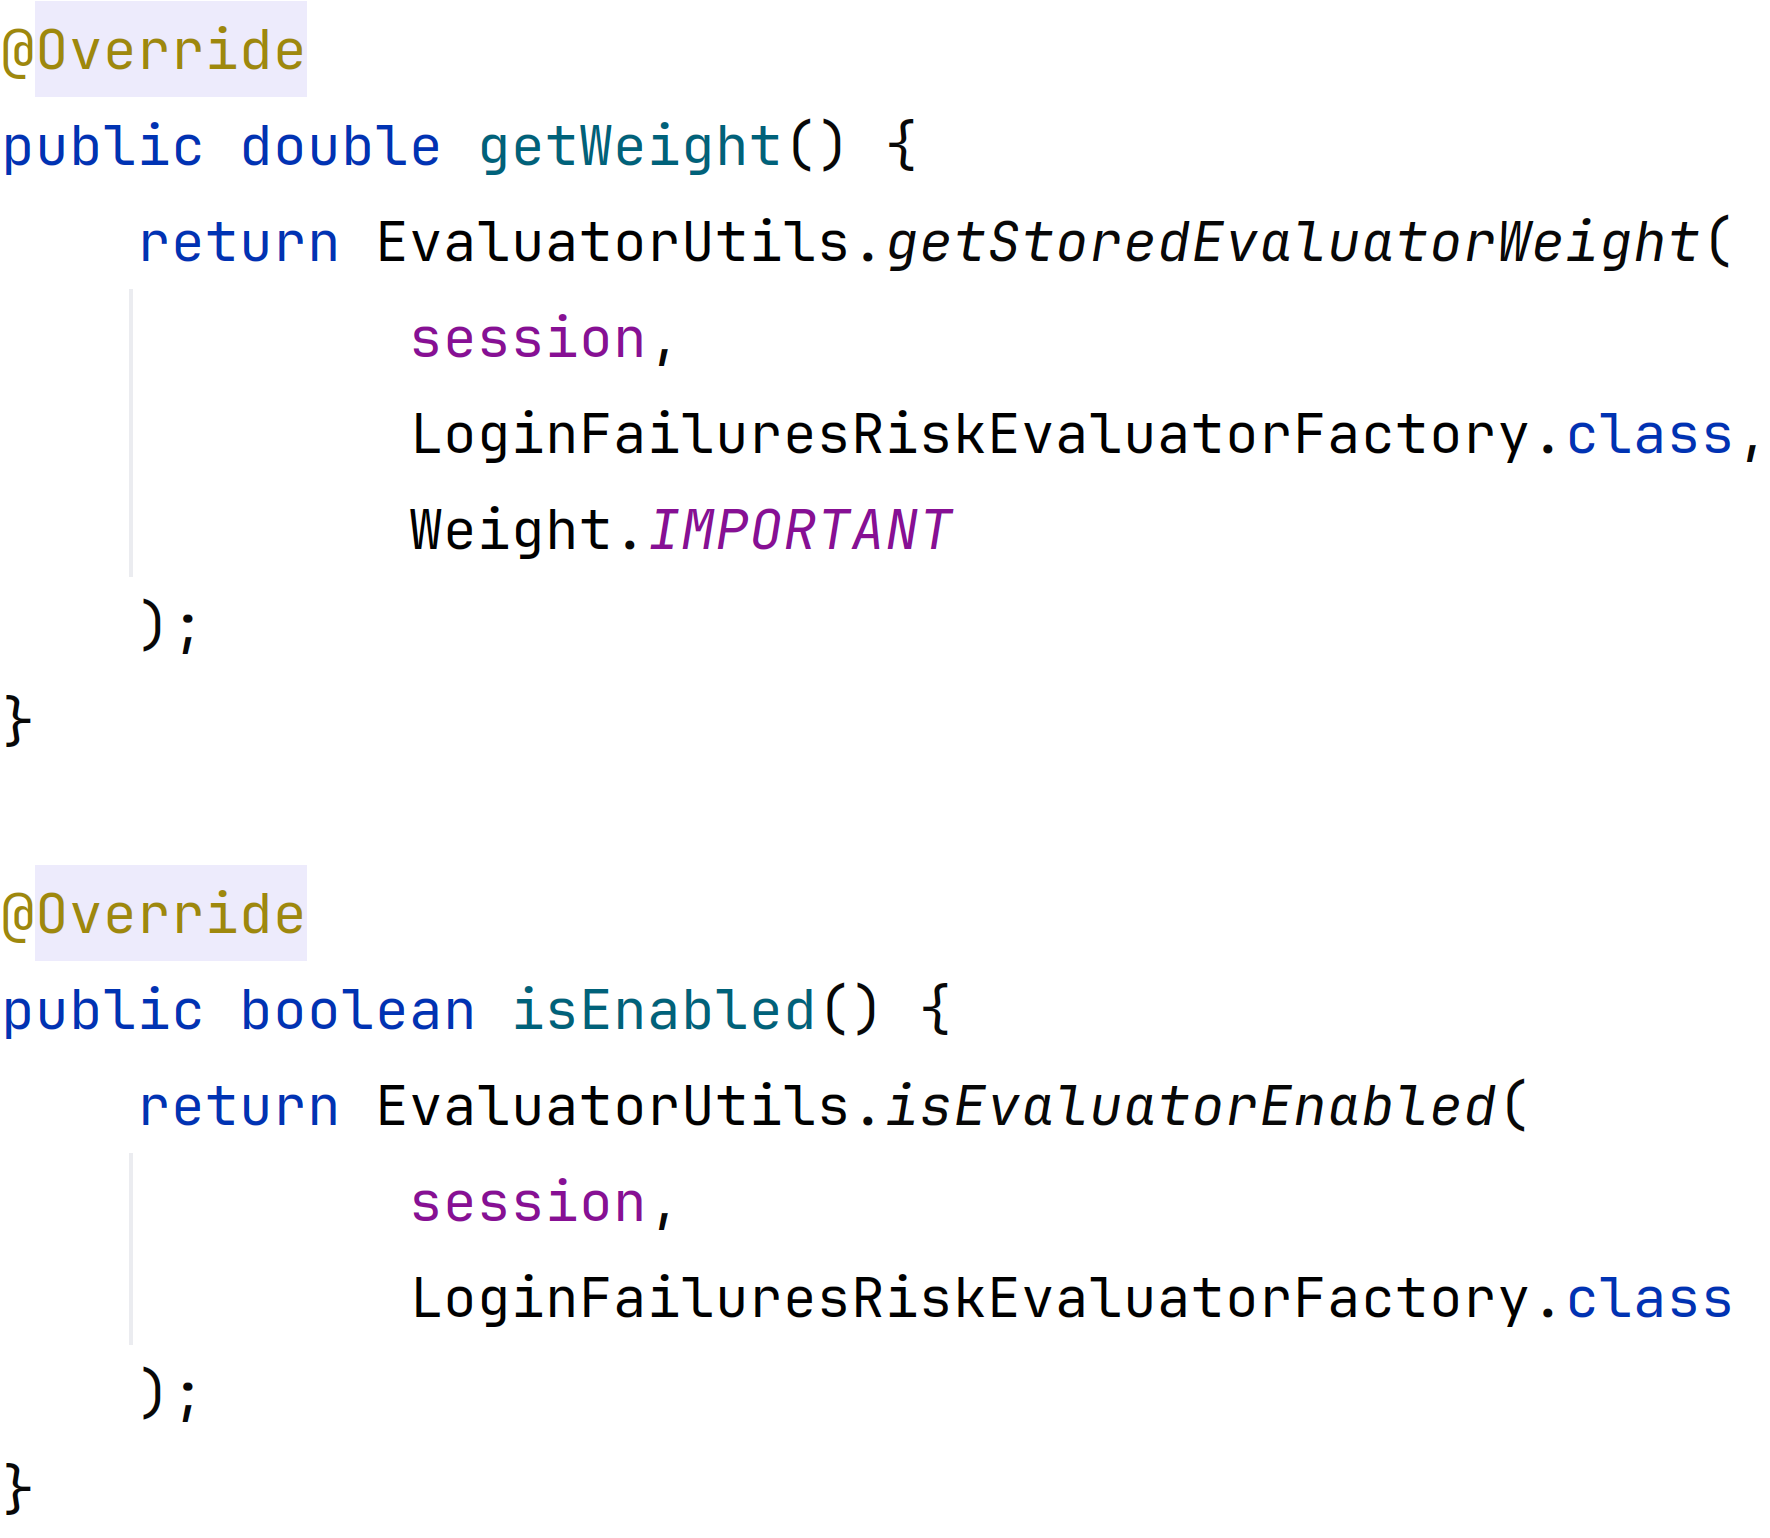
\includegraphics[width=0.6\textwidth]{img/sections/6-implementation/loginFailuresConfig.png}
  \caption{Login Failures Risk Evaluator Configuration}
  \label{fig:impl-risk-evaluator-login-failures-config}
\end{figure}

\newpage
\section{User Engine}
\subsection{Asynchronous processing}
\subsection{Evaluation}
\subsection{Store Risk Score}

\newpage
\section{Artificial Intelligence}

\newpage
\section{External Integration}

\shorthandoff{-}